\begin{figure*}[!t]
    \centering
    % \scalebox{0.9}{
    \subfloat[\scriptsize{Chemprot}]{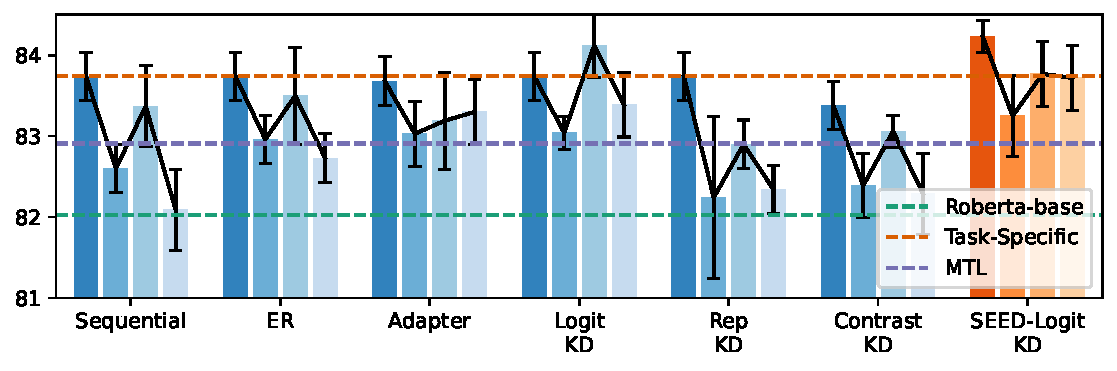
\includegraphics[width=0.48\linewidth]{acl2022/figs/academics_plots/Chemprot.pdf}}
    \subfloat[\scriptsize{RCT-Sample}]{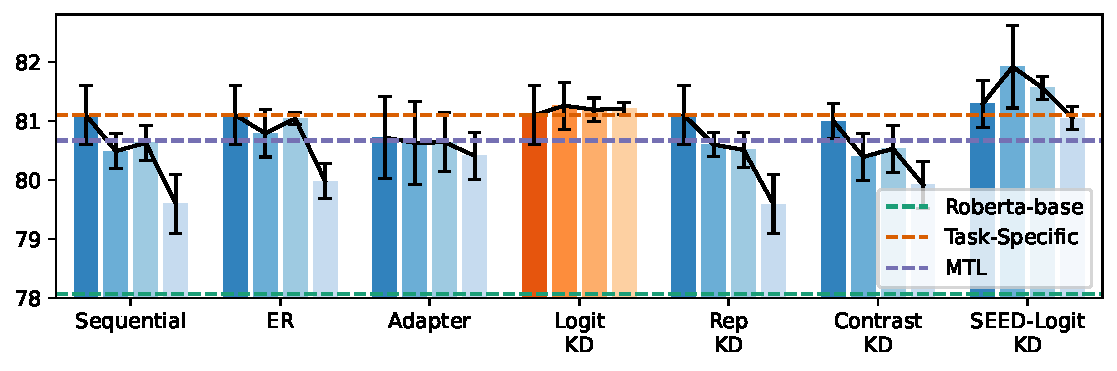
\includegraphics[width=0.48\linewidth]{acl2022/figs/academics_plots/RCT-Sample.pdf}}


    \subfloat[\scriptsize{ACL-ARC}]{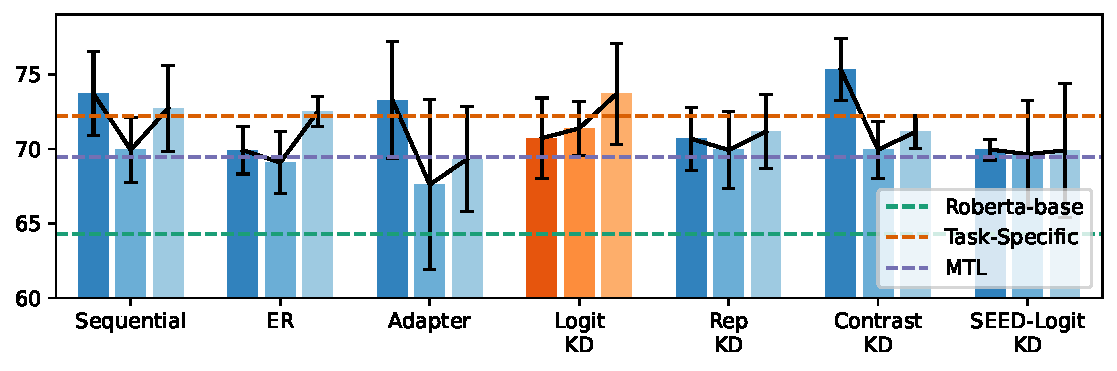
\includegraphics[width=0.48\linewidth]{acl2022/figs/academics_plots/ACL-ARC.pdf}}
    \subfloat[\scriptsize{SciERC}]{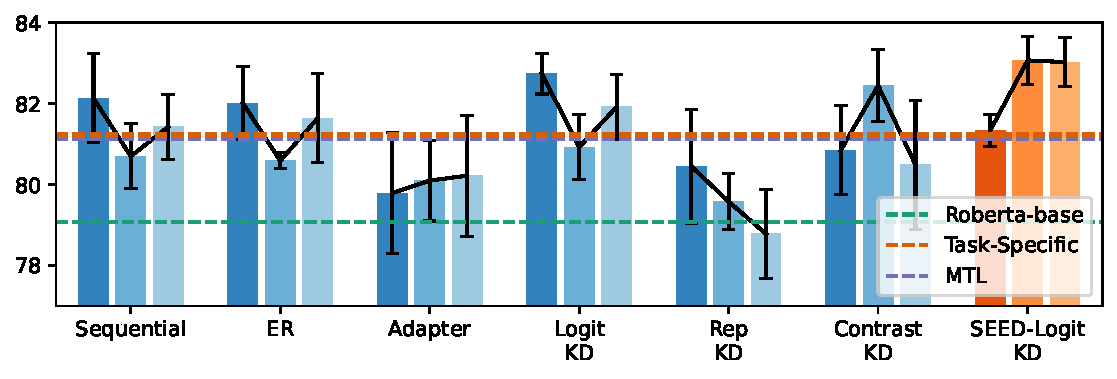
\includegraphics[width=0.48\linewidth]{acl2022/figs/academics_plots/SciERC.pdf}}
    % }
    \caption{\small \textbf{Performance evolution of downstream models.} Models are fine-tuned from checkpoints of lifelong pretrained LMs at different time steps $t$. For Chemprot and RCT-Sample from $D_1$, we use $t \in \{1,2,3,4\}$; while for ACL-ARC and SciERC from $D_2$, $t \in \{2,3,4\}$. Methods achieving the best performance at the end of training ($t=4$) is highlighted.}
    \label{fig:academics_curve}
    \vspace{-0.3cm}
\end{figure*}